\documentclass[conference]{IEEEtran}
\IEEEoverridecommandlockouts
% The preceding line is only needed to identify funding in the first footnote. If that is unneeded, please comment it out.
\usepackage{cite}
\usepackage{amsmath,amssymb,amsfonts}
\usepackage{algorithmic}
\usepackage{graphicx}
\graphicspath{ {images/} }
\usepackage{textcomp}
\def\BibTeX{{\rm B\kern-.05em{\sc i\kern-.025em b}\kern-.08em
    T\kern-.1667em\lower.7ex\hbox{E}\kern-.125emX}}
\begin{document}

\title{Automatic Medical Coding for Neonatal Jaundice with Machine Learning
}


\author{\IEEEauthorblockN{Scott Werwath}
\IEEEauthorblockA{
\textit{UC Berkeley}\\
sbw@berkeley.edu}
}

\maketitle

\begin{abstract}
This study explores the creation of a machine learning model to automatically identify whether a Neonatal Intensive Care Unit (NICU) patient was diagnosed with neonatal jaundice during a particular hospitalization based on their associated clinical notes. We develop a number of techniques for text preprocessing and feature selection and compare the effectiveness of different classification models. 
\end{abstract}

\section{Introduction}
\subsection{Medical Coding}\label{AA}
In the course of normal clinical operations, healthcare providers are often required to \textit{code} patient records. The process of coding involves taking all data associated with a single patient case and abstracting out a set of standardized alphanumeric codes where each unique code is associated with a unique diagnosis or medical procedure. These codes are used for a variety of applications, including medical billing, as labels in statistical analysis of medical datasets, as features in clinical decision making, and as tags in information retrieval systems. 

While many coding schemes exists, the most widely used is the International Classification of Diseases, 9\textsuperscript{th} Revision (ICD-9) [SLEE]. Each ICD-9 codes consists of 3 to 5 alphanumeric characters which represents either a diagnosis or a procedure.

In actual clinical practice, coding is performed manually by professional medical coders. This process is both time-intensive and error-prone due to the fact that patient health records contain a large amount of data in free-text narrative format which is difficult to interpret quickly for both humans and computers [TANGE]. 

A system for automatic coding would have the potential to substantially decrease the number of man-hours required to process clinical cases, but building such a system requires the ability to extract important information from free-text reports. To this end, the application of natural language processing (NLP) and machine learning (ML) techniques to clinical texts show much promise [MEYSTRE].

\subsection{Neonatal Jaundice}\label{AA}
Neonatal jaundice, also called neonatal hyperbilirubinemia, is a yellow discoloration of the skin due to elevated bilirubin in a neonate's (infant's) blood. Transient neonatal jaundice is somewhat common in infants and usually carries little risk. However, untreated jaundice can put premature or otherwise ill infants at great risk of developing permanent neurological impairments [LANTZY]. Additionally, it has been shown that the diagnosis of neonatal jaundice is a risk factor for both mortality and rehospitalization [ESCOBAR]. 

Both the risk factors associated with and the relative prevalence of neonatal jaundice make it an excellent subject for study using machine learning techniques; the risk factors provide the motivation, while the prevalence provide a wealth of data to be analyzed.

\section{Related Work}
The past few years have seen a meteoric rise in the application of natural language processing (NLP) in the medical field [WOLNIEWICZ]. The cost of analyzing medical documents, both monetary and time, has motivated efforts to automate many manual tasks in the analysis and processing of medical texts.

Given both the importance and time-intensive nature of medical coding, many scientists have started developing techniques for automated coding. [MEYSTRE]. For most of these attempts, the task was domain-specific (i.e. attempting to predict a single ICD code or a small set of related codes) and utilized a relatively small dataset. 

At least one attempt has been made to use deep learning (namely character-level recurrent neural networks) to build more general coding models, but with limited success [SHI]. The main limitation with this method is that deep learning models require a large amount of data to train [CHEN], but even a large clinical dataset may only contain a few examples of case files with any given ICD code. Additionally, since the ICD-9 standard contains over 14,000 different codes. Treating coding as a simple multi-class classification problem with 14,000 different classes is infeasible.

More successful automated coding models have utilized non-deep machine learning techniques such as support vector machines (SVMs) [VAPNIK] and focus on training a model to detect the presence of a single ICD code or class of related codes. Some of these methods also leverage structured data stored in health records in addition to free-text narratives [FERRAO].

At least one previous attempt has been made to build an automatic coding model for neonatal jaundice using an SVM on the text of clinical notes [MARAFINO]. Our research improves on this model by introducing a number of preprocessing stages. We also explore and compare alternative classification techniques and analyze their efficacy.

No matter the exact method for extracting medical codes from free-text, two common NLP challenges must be solved. First, one must represent free-text in an appropriate feature space (usually as a vector). Second, one must train a model to accurately classify patient records based on the selected features. 

\section{Methodology}
\subsection{Dataset and Data Extraction}\label{AA}
The Medical Information Mart for Intensive Care III (MIMIC-III) dataset contains complete anonymized records from over 53,000 ICU stays [JOHNSON]. These records were gathered from hospital records from the Beth Israel Deaconess Medical Center in Boston, Massachusetts between 2001 and 2012. Of these records, 7870 correspond to neonates admitted between 2001 and 2008. 

Each hospital stay in the MIMIC-III dataset is assigned a unique HADM\_ID identifier which can be used to cross-reference associated data back their associated hospitalization.

In order to find all patients who were diagnosed with neonatal jaundice, we found all HADM\_IDs that were labeled with an ICD-9 code associated with neonatal jaundice. A list of such codes are shown in Table~\ref{tab1}. 
\begin{table}[htbp]
\caption{ICD-9 Codes for Neonatal Jaundice}
\begin{center}
\begin{tabular}{cc}
\textbf{ICD-9 Code}&\textbf{Description} \\
\hline
\textbf{773.0} & Hemolytic disease, RH isoimmunization \\
\textbf{773.1} & Hemolytic disease, ABO isoimmunization \\
\textbf{773.0} & Hemolytic disease, unknown \\
\textbf{774.1} & Perinatal jaundice, excessive hemolysis \\
\textbf{774.2} & Neonatal jaundice, preterm delivery \\
\textbf{774.30} & Neonatal jaundice, delayed conjugation \\
\textbf{774.31} &  Neonatal jaundice, delayed conjugation, other \\
\textbf{774.39} & Other jaundice \\
\textbf{774.6} & Unspecified fetal and neonatal jaundice \\
\end{tabular}
\label{tab1}
\end{center}
\end{table}
In total, 7092 hospitalizations were of neonates. Of these, 2868 stays were associated with a neonatal jaundice diagnosis and served as positive examples. We also selected the remaining 4224 non-jaundice NICU stays as negative examples.

For each relevant hospitalization, we concatenated all ICU notes, including nursing notes, radiology reports, physician progress notes, and discharge summaries into a single string of text called a \textit{noteset}. This string served as the raw data to be preprocessed and then classified. 
\subsection{Data Preprocessing}\label{AA}

\subsection{Document Representation}\label{AA}

\subsection{Classification Models}\label{AA}

\subsection{Evaluation}\label{AA}

Number equations consecutively. To make your 
equations more compact, you may use the solidus (~/~), the exp function, or 
appropriate exponents. Italicize Roman symbols for quantities and variables, 
but not Greek symbols. Use a long dash rather than a hyphen for a minus 
sign. Punctuate equations with commas or periods when they are part of a 
sentence, as in:
\begin{equation}
a+b=\gamma\label{eq}
\end{equation}

Be sure that the 
symbols in your equation have been defined before or immediately following 
the equation. Use ``\eqref{eq}'', not ``Eq.~\eqref{eq}'' or ``equation \eqref{eq}'', except at 
the beginning of a sentence: ``Equation \eqref{eq} is . . .''

\section{Results}
\subsection{Performance of TF-IDF Methods}\label{AA}
\subsection{Evaluation}\label{AA}


\section{Conclusion}
Headings, or heads, are organizational devices that guide the reader through 
your paper. There are two types: component heads and text heads.

Component heads identify the different components of your paper and are not 
topically subordinate to each other. Examples include Acknowledgments and 
References and, for these, the correct style to use is ``Heading 5''. Use 
``figure caption'' for your Figure captions, and ``table head'' for your 
table title. Run-in heads, such as ``Abstract'', will require you to apply a 
style (in this case, italic) in addition to the style provided by the drop 
down menu to differentiate the head from the text.

Text heads organize the topics on a relational, hierarchical basis. For 
example, the paper title is the primary text head because all subsequent 
material relates and elaborates on this one topic. If there are two or more 
sub-topics, the next level head (uppercase Roman numerals) should be used 
and, conversely, if there are not at least two sub-topics, then no subheads 
should be introduced.

\subsection{Figures and Tables}
\paragraph{Positioning Figures and Tables} Place figures and tables at the top and 
bottom of columns. Avoid placing them in the middle of columns. Large 
figures and tables may span across both columns. Figure captions should be 
below the figures; table heads should appear above the tables. Insert 
figures and tables after they are cited in the text. Use the abbreviation 
``Fig.~\ref{fig}'', even at the beginning of a sentence.

\begin{table}[htbp]
\caption{Table Type Styles}
\begin{center}
\begin{tabular}{|c|c|c|c|}
\hline
\textbf{Table}&\multicolumn{3}{|c|}{\textbf{Table Column Head}} \\
\cline{2-4} 
\textbf{Head} & \textbf{\textit{Table column subhead}}& \textbf{\textit{Subhead}}& \textbf{\textit{Subhead}} \\
\hline
copy& More table copy$^{\mathrm{a}}$& &  \\
\hline
\multicolumn{4}{l}{$^{\mathrm{a}}$Sample of a Table footnote.}
\end{tabular}
\label{tab2}
\end{center}
\end{table}

\begin{figure}[htbp]
\centerline{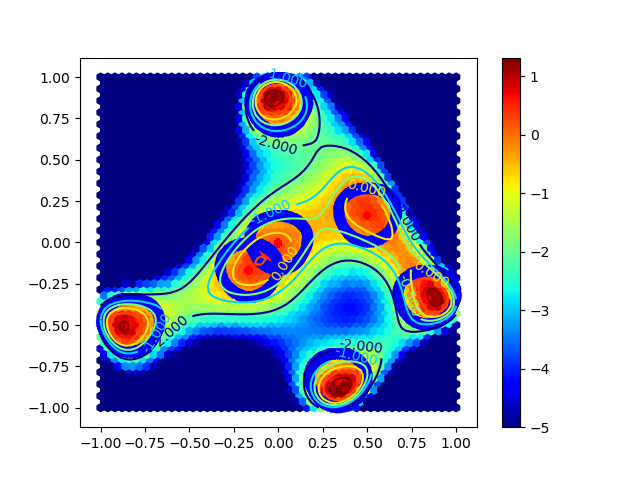
\includegraphics[scale=0.5]{fig1}}
\caption{Example of a figure caption.}
\label{fig}
\end{figure}

Figure Labels: Use 8 point Times New Roman for Figure labels. Use words 
rather than symbols or abbreviations when writing Figure axis labels to 
avoid confusing the reader. As an example, write the quantity 
``Magnetization'', or ``Magnetization, M'', not just ``M''. If including 
units in the label, present them within parentheses. Do not label axes only 
with units. In the example, write ``Magnetization (A/m)'' or ``Magnetization 
\{A[m(1)]\}'', not just ``A/m''. Do not label axes with a ratio of 
quantities and units. For example, write ``Temperature (K)'', not 
``Temperature/K''.

\section*{Acknowledgment}

The preferred spelling of the word ``acknowledgment'' in America is without 
an ``e'' after the ``g''. Avoid the stilted expression ``one of us (R. B. 
G.) thanks $\ldots$''. Instead, try ``R. B. G. thanks$\ldots$''. Put sponsor 
acknowledgments in the unnumbered footnote on the first page.

\section*{References}

Please number citations consecutively within brackets \cite{b1}. The 
sentence punctuation follows the bracket \cite{b2}. Refer simply to the reference 
number, as in \cite{b3}---do not use ``Ref. \cite{b3}'' or ``reference \cite{b3}'' except at 
the beginning of a sentence: ``Reference \cite{b3} was the first $\ldots$''

Number footnotes separately in superscripts. Place the actual footnote at 
the bottom of the column in which it was cited. Do not put footnotes in the 
abstract or reference list. Use letters for table footnotes.

Unless there are six authors or more give all authors' names; do not use 
``et al.''. Papers that have not been published, even if they have been 
submitted for publication, should be cited as ``unpublished'' \cite{b4}. Papers 
that have been accepted for publication should be cited as ``in press'' \cite{b5}. 
Capitalize only the first word in a paper title, except for proper nouns and 
element symbols.

For papers published in translation journals, please give the English 
citation first, followed by the original foreign-language citation \cite{b6}.

\begin{thebibliography}{00}
\bibitem{b1} G. Eason, B. Noble, and I. N. Sneddon, ``On certain integrals of Lipschitz-Hankel type involving products of Bessel functions,'' Phil. Trans. Roy. Soc. London, vol. A247, pp. 529--551, April 1955.
\bibitem{b2} J. Clerk Maxwell, A Treatise on Electricity and Magnetism, 3rd ed., vol. 2. Oxford: Clarendon, 1892, pp.68--73.
\bibitem{b3} I. S. Jacobs and C. P. Bean, ``Fine particles, thin films and exchange anisotropy,'' in Magnetism, vol. III, G. T. Rado and H. Suhl, Eds. New York: Academic, 1963, pp. 271--350.
\bibitem{b4} K. Elissa, ``Title of paper if known,'' unpublished.
\bibitem{b5} R. Nicole, ``Title of paper with only first word capitalized,'' J. Name Stand. Abbrev., in press.
\bibitem{b6} Y. Yorozu, M. Hirano, K. Oka, and Y. Tagawa, ``Electron spectroscopy studies on magneto-optical media and plastic substrate interface,'' IEEE Transl. J. Magn. Japan, vol. 2, pp. 740--741, August 1987 [Digests 9th Annual Conf. Magnetics Japan, p. 301, 1982].
\bibitem{b7} R. Wolniewicz (2015). "Computer-assisted coding and natural language processing."
\end{thebibliography}

\end{document}
